% FPGA case studies section for tech report

\subsection{Eight-Tap Filter}

An 8-tap direct-form FIR was implemented in Verilog for three coefficient
sets: A (all 16-bit), B (all 8-bit), and C ($[4,16,8,8,8,8,16,4]$).
Bit-exact integer-reference simulation covered 157 cycles with zero
mismatches for all three configurations.

Six synthesis/implementation runs (A1/A2, B1/B2, C1/C2; forced-DSP and
auto-mapping) were completed on XC7A35T-2FGG484 with Vivado 2022.2.2
using a 10\,ns clock and assumed 2\,ns I/O delays. Table~\ref{tab:fpga8}
reports routed resources.

\begin{table}[!t]
\caption{Eight-tap routed FPGA resources (corrected RTL)}
\label{tab:fpga8}
\centering
\scriptsize
\begin{tabular}{l r r r r r}
\toprule
Run & DSP & LUT$_\text{logic}$ & LUT$_\text{mem}$ & FF & Core WNS (ns)\\
\midrule
A1/A2 & 8 & 100 & 0 & 109 & 5.952\\
B1 & 6 & 124 & 0 & 189 & 6.500\\
B2 & 4 & 166 & 16 & 279 & 6.725\\
C1/C2 & 6 & 132 & 0 & 175 & 6.323\\
\bottomrule
\end{tabular}
\end{table}

Core register-to-register WNS is positive in all runs; overall WNS is
negative ($-0.213$ to $-0.695$\,ns) on paths ending at output ports under
assumed 2\,ns output delay. These are not board-level timing signoff
results. FIR-only DRC reports NSTD-1 and UCIO-1 Critical Warnings on
unconstrained top-level ports.

\textbf{Board verification.} Three bitstream configurations (A, B, C)
were programmed to a legacy ACX750 development board (XC7A35T-2FGG484)
via JTAG. UART-paced testing delivered the same 157-sample input sequence
to each configuration; each was freshly programmed and tested twice.
Across 3 configurations $\times$ 2 runs $\times$ 157 samples = 942
bit-exact comparisons against integer-precision reference values, zero
mismatches were observed. This establishes functional correctness under
the tested operating point; it does not measure maximum frequency,
throughput, or power.

The 8-tap datapath uses signed 16-bit samples with 14 fractional bits.
A $w$-bit signed coefficient has $w-1$ fractional bits; its $16+w$-bit
product is sign-extended to 32 bits and left-shifted by $16-w$ to
29 fractional bits. The three registered adder levels use 33, 34, and
35 bits, respectively. The reference model specifies a five-cycle valid
delay. The RTL performs no saturation or fractional rounding in this
path; fixed-width overflow wraps. Input and coefficient quantization
in the reference preparation uses rounding and clipping to representable
ranges. These details concern functional validation, not measured Fmax.

\subsection{Forty-Eight-Tap Filter}

A 48-tap equiripple low-pass FIR (passband 0--0.3$\pi$, stopband
0.4$\pi$--$\pi$, $\pm$0.25\,dB passband, $\le -40$\,dB stopband) was
designed with MATLAB \texttt{firpm}. For quota $[24,16,8]$, the DP
allocation has coefficient SSE $1.8594 \times 10^{-5}$ and a computed
stopband peak of $-41.30$\,dB (meets the $-40$\,dB limit); a same-quota
greedy allocation has SSE $6.6658 \times 10^{-5}$ and $-35.78$\,dB
(fails). Two other quotas ($[16,24,8]$ and $[12,24,12]$) fail the
stopband limit even under DP, showing that coefficient-SSE optimality
does not guarantee spectral compliance.

Quotas count the 48 coefficient positions before folding. The allocators
do not impose paired-width constraints: for quota $[24,16,8]$, the DP
allocation has two mirror pairs with different width labels (1/48 and
4/45), and greedy has six (1/48, 2/47, 4/45, 5/44, 7/42, and 10/39).
In every such pair both quantized values are zero. After fixed
point alignment the quantized vectors are therefore exactly mirror
symmetric (maximum mirror error zero), which is the condition used by
the folded RTL. The RTL generator checks this before emitting the folded
design. Each shared product uses the width and stored constant of the
first member of the pair (positions 1--24); mismatched mirror labels
only occur for zero values. The folded datapath uses 24 pair sums and 24 coefficient
products; the reported quota remains the pre-fold count.

Figure~\ref{fig:response48} compares the computed responses for the first
quota. Both allocations meet the passband limit, but only DP meets the
stopband limit in this case.

\begin{figure}[!t]
\centering
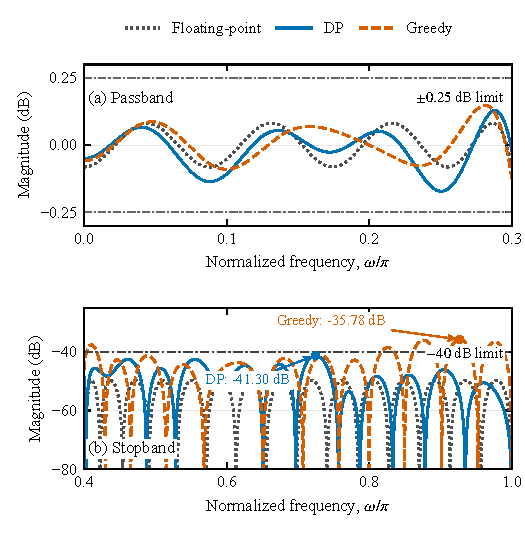
\includegraphics[width=\columnwidth]{figures/frequency_response_quota1.pdf}
\caption{Computed frequency responses of the 48-tap FIR for quota
$[24,16,8]$: (a) passband detail and (b) stopband detail. Gray dash-dot
lines mark the stated limits. DP and greedy stopband peaks are
$-41.30$ and $-35.78$\,dB, respectively. These curves are calculated
from the saved coefficients, not measured on hardware.}
\label{fig:response48}
\end{figure}

Eight RTL variants (DP, greedy, uniform 16-bit, uniform 8-bit; direct
and symmetric-folded) passed XSim simulation over 2,500 cycles with
1,861 valid outputs per design (14,888 total output comparisons) against
an independent 48-term integer-convolution reference. Four
symmetric-folded and direct-form routes were completed on the same
XC7A35T part. Table~\ref{tab:fpga48} reports routed resources for the
DP and greedy symmetric-folded designs.

The tested RTL uses signed 16-bit input samples with 14 fractional bits
and signed coefficient words with one sign bit and $w-1$ fractional bits.
Folded products use a signed 17-bit pair sum. Products and every registered
partial-sum node at tree levels 1--5 are signed 38-bit values with 29
fractional bits; the output is the signed 38-bit value at level 5, also
with 29 fractional bits (9 remaining sign/integer bits). Product alignment
uses exact left shifts, with no rounding or saturation; fixed-width
overflow wraps. The generated vectors remain within the representable
38-bit output range. The eight registered arithmetic stages give a
seven-edge accepted-input to valid-output difference in the testbench.
These statements describe the tested RTL and are not a general resource
model for arbitrary widths.

\begin{table}[!t]
\caption{Forty-eight-tap routed resources for quota $[24,16,8]$}
\label{tab:fpga48}
\centering
\scriptsize
\resizebox{\columnwidth}{!}{%
\begin{tabular}{l r r r r r r}
\toprule
Design & DSP & LUT$_L$ & LUT$_M$ & Slice LUT & FF & Reg--reg (ns)\\
\midrule
DP, folded & 21 & 322 & 32 & 354 & 1066 & 4.344\\
Greedy, folded & 21 & 200 & 16 & 216 & 997 & 5.189\\
DP, direct & 38 & 654 & 80 & 734 & 1106 & 5.763\\
Greedy, direct & 39 & 412 & 64 & 476 & 1043 & 4.879\\
\bottomrule
\end{tabular}}
\vspace{1mm}
\parbox{\columnwidth}{\scriptsize Overall WNS (row order):
$-0.213$, $-0.430$, $-0.435$, $-0.213$\,ns. Negative WNS on assumed
output-delay paths.}
\end{table}

The response-compliant DP allocation uses more slice LUTs (354 vs.\ 216)
and flip-flops (1066 vs.\ 997) than the non-compliant greedy allocation;
this is a bounded resource--response tradeoff for one filter and one
quota, not a general superiority claim. No 48-tap board test, measured
Fmax, sustained throughput, or power measurement was performed.
